\documentclass[12pt, a4paper]{article}
\usepackage[utf8]{inputenc}
\usepackage{geometry}
\geometry{left=1in, right=1in, top=1in, bottom=1in}
\usepackage{amsmath, amssymb, amsfonts} 
\usepackage{graphicx} 
\usepackage[margin=1in]{geometry}
\usepackage{booktabs}
\usepackage{natbib}
\usepackage{setspace}
\usepackage{hyperref}
\usepackage{float}
\usepackage{caption}
\usepackage{subcaption}
\usepackage{enumitem}
\usepackage{threeparttable}
\usepackage{caption}
\usepackage{subcaption}
\usepackage{placeins}

\title{\textbf{Tax Capitalisation in the UK Used Car Market: Evidence from UK Vehicle Excise Tax Reform with the case of Toyota}}
\author{Emma (Sunwoo) Cho \\ 
\small University of South Carolina \\
\small \texttt{emmacho@sc.edu}}
\date{December 9, 2025}

\begin{document}
\maketitle

\begin{abstract}
The purchase of an automobile typically depends not only on the vehicle’s purchase price but also on its expected operating costs. This study examines how consumers capitalise future tax liabilities into used car prices, leveraging the exogenous reform of the UK Vehicle Excise Duty (VED) in April 2017 as a natural experiment. Prior to the reform, annual road taxes varied substantially by $CO_{2}$ emissions; post-reform, most vehicles face a flat rate (a lump-sum tax scheme), creating a structural break in expected operating costs for automobile consumers. Using a Toyota used-car dataset, I employ a Simulated Method of Moments (SMM) approach combined with a structural pricing model to estimate consumer tax capitalisation and its effect on used-car prices, which may further influence consumer choice. The results indicate a tax capitalisation coefficient ($\lambda$) of approximately 1.13, suggesting that consumers fully (and potentially over-) capitalise future tax savings into current vehicle prices. These findings show a significant change in consumer behavior corresponding to the VED reform in the UK used-car market; although the evidence is based on a single brand only, it may shed light and provide preliminary evidence for further exploration of the impact of this type of tax scheme change on consumer choice.

\vspace{0.5cm}
\noindent \textbf{Keywords:} Tax capitalisation, Structural Estimation, Vehicle Excise Duty, Used Car Market, Used Car Price, Durable Goods, Toyota
\end{abstract}

\thispagestyle{empty} % no page number on title page
\newpage
\setcounter{page}{1}
\onehalfspacing % 1.5 Line spacing 

\section{Introduction}
The valuation of long-term costs from consumer perspective is an important question to address in the intersection of public economics and industrial organization \citep{grigolon2018, allcott2014, sallee2016, chetty2009}. This can be also important to in the marketing field that is useful to expect the consumer behavior dynamics. When purchasing durable goods like automobiles, rational consumers should consider not only the purchase price but also take into account of future operating cost, and if assumed consumers to be rational, this should be the present discounted value of future operating costs, including taxes \citep{grigolon2018, allcott2014, sallee2016}. 
In theory, if consumers are forward-looking and rational, these future costs should be fully reflected in market prices. However, on the other hand, behavioral economics prior research suggests that tax salience (whether consumers actually notice the tax change and mentally process its effect when making the consuequence decision or future expectations), myopia, and cognitive limitations of taking these all account, may lead to incomplete capitalisation and not significant impact of consumer purchase decision \citep{chetty2009, finkelstein2009}.

Thus, to provide empirical evidence on this question, this paper leverages an exogenous policy revision with a unique institutional structure: the April 2017 reform of the UK Vehicle Excise Duty (VED). Prior to 2017, VED operated as a granular Pigouvian tax scheme system, with annual tax liability being a finely classified based on a vehicle’s specific $CO_{2}$ emissions. In April 2017, the regime implemented to a new flat-rate system, converting the tax from a marginal cost on emissions into a standardised lump-sum fee on ownership of vehicle itself. This structural break event provides a possible quasi-experimental setting. The pre-2017 system closely resembles the environmentally oriented tax schemes that many recent policies seek to introduce, whereas the 2017 reform was explicitly a fiscal correction designed to stabilise revenue and, in doing so, decoupled the tax from its environmental purpose, which sounds counter to the sustainability trend that recently get a huge attention. This creates a unique opportunity to study how markets react when a policy’s primary objective shifts from correcting externalities to generating revenue. By leveraging this variation, this paper examines the extent to which the UK VED is capitalised into used car prices and, in doing so, provides structural evidence on how the design of tax policy (and its trade-off between fiscal stability and environmental incentives) shapes consumer asset valuation. This structural break offers a distinct advantage for identification. It allows us to observe how valuation changes when the tax regime simplifies from a complex classified system (that was aiming for sustainability of the society) to a salient, uniform cost. Using a dataset of Toyota vehicles and employing a structural estimation framework (Simulated Method of Moments, SMM), I estimate the rate of tax capitalisation. The structural approaches enaable to find parameter estimates of importance in theory that governing consumer preferences for tax savings versus vehicle depreciation. 

My main findings are as follows. Using a Simulated Method of Moments (SMM) estimation, I estimate a tax capitalisation coefficient of $\lambda \approx 0.95$, implying that consumers fully capitalise future tax liabilities into used car prices. I reject the null hypothesis of no capitalisation but am not able to reject full capitalisation. Additionally, a heterogeneity analysis using machine learning reveals that the 2017 reform created asymmetric effects: high-emission vehicles gained value, while low-emission vehicles lost their tax advantage.

This paper makes important contributions to several literatures. First, it adds to the tax capitalisation literature \cite{oates1969, busse2006} by providing structural estimates in an automotive context. While previous studies have examined property taxes and sales taxes, less is known about how recurring ownership taxes are capitalised into durable goods prices. Second, it contributes to the literature on hedonic pricing \cite{rosen1974, berry1995} by estimating consumer valuations in the used car market using a structural approach. Lastly, my findings inform environmental tax policy design by demonstrating how the shift from emissions-based to flat-rate taxation affected secondary-market durable goods' valuations that especially involving the operational costs to maintain the goods.

The remainder of this paper is organized as follows. Section 2 describes the institutional background of UK vehicle taxation. Section 3 explains the data and summary statistics of it. Section 4 develops the theoretical framework and estimation strategy. Section 5 presents the empirical results, and Section 6 concludes with policy implications and discussion.

\section{Institutional Background}
The UK Vehicle Excise Duty (VED) is an annual tax levied on vehicle ownership. For most of the 20th century, VED rates were based on engine size, with a simple two-tier structure. However, following the 1997 election, the Labour Party under Chancellor Gordon Brown sought to use the tax system to incentivise fuel-efficient vehicles as part of broader climate commitments. In the 1999 Budget, Brown announced a new emissions-based VED system, implemented from March 2001. Under this regime, vehicles were assigned to one of 13 bands (A through M) based on CO\textsubscript{2} emissions. Low-emission vehicles in Band A (below 100 g/km) paid \pounds 0 annual tax, while high-emission vehicles in Bands K--M (above 200 g/km) faced charges of \pounds 290--500 or more. This system created strong purchase incentives: fuel-efficient hybrids such as the Toyota Prius qualified for tax-exempt status, while sports cars and SUVs faced substantial annual liabilities \citep{ukbudget1999, dvla2001, CerrutiAlberiniLinn2017}.

By 2015, however, the environmental success of the CO\textsubscript{2}-based system had created a fiscal problem. As vehicles became more efficient, the proportion falling into tax-exempt or low-tax bands grew substantially. Government projections showed VED revenue declining from \pounds 4.4 billion in 2015 to under \pounds 3 billion by 2020--21. The UK Government addressed this in the Summer Budget 2015 speech: “Because so many new cars now fall into the low-carbon emission bands, by 2017 over three quarters of new cars will pay no VED at all in the first year.” The reform faced several conflicts among stakeholders before being passed. Nevertheless, in response to the stated problem, the Government announced a fundamental restructuring of VED, implemented from April 1, 2017. Under the new system, first-year rates still vary by CO\textsubscript{2} emissions (ranging from \pounds 0 to over \pounds 2,000), but from the second year onward nearly all vehicles pay a flat standard rate of approximately \pounds 145 regardless of emissions. An additional premium supplement of \pounds 310 per year applies to vehicles with list prices exceeding \pounds 40,000 \citep{hmt2015, dvla2015, dvla2017}.

The 2017 reform created an exogenous shock, making the difference in tax liability depend solely on registration date and eliminating the environmental-benefit structure of the previous system. Two mechanically identical vehicles (same model, same engine, same emissions) face vastly different lifetime tax liabilities (and expected operating costs) depending on whether registration occurred before or after April 1, 2017. This discontinuity is illustrated in Table \ref{tab:tax_discontinuity} for two Toyota models, the single brand examined in this study. Using this identification opportunity, this paper finds that low-emission vehicles like the Prius lost their tax advantage under the flat-rate system, while high-emission vehicles such as the GT86 effectively received tax relief.

%If consumers capitalise future taxes into prices, we should observe post-2017 hybrids trading at a discount and post-2017 sports cars trading at a premium relative to their pre-2017 counterparts, conditional on age and other characteristics.

\begin{table}[H]
\centering
\caption{Tax Liability by Registration Date Example for Two Models}
\label{tab:tax_discontinuity}
\begin{tabular}{lccc}
\toprule
Vehicle Type & Pre-April 2017 & Post-April 2017 & 5-Year Difference \\
\midrule
Toyota Prius (Hybrid) & \pounds 0/year & \pounds 135/year & +\pounds 675 \\
Toyota GT86 (Sports) & \pounds 265/year & \pounds 145/year & $-$\pounds 600 \\
\bottomrule
\end{tabular}
\end{table}

\section{Data}

I use a dataset of used Toyota car listings from the UK market, obtained from a publicly available Kaggle repository. The original dataset contains 6,738 observations of Toyota vehicles listed for sale, covering model years from 1998 to 2020. Each observation represents an individual vehicle listing and includes information on the listing price, model name, year of first registration, mileage (odometer reading), transmission type, fuel type, engine size, MPG (fuel efficiency), and annual VED amount.

The dependent variable is the listing price in British pounds. Prices in the sample range from \pounds 850 to \pounds 59,995, with a mean of \pounds 12,522 and substantial variation (standard deviation of \pounds 6,345), reflecting the heterogeneity of vehicle types and ages in the used car market. The main independent variable of interest is the annual VED amount, which ranges from \pounds 0 (for pre-2017 low-emission vehicles qualifying for Band A) to \pounds 565 (for high-emission vehicles in the upper bands). The mean tax of \pounds 94.7 with a standard deviation of \pounds 73.9 indicates considerable cross-sectional variation, which is essential for identifying the capitalisation coefficient.

The dataset includes 15 distinct Toyota models spanning various market segments: economy vehicles (Aygo, Yaris), family cars (Corolla, Auris, Avensis), hybrids (Prius), crossovers and SUVs (C-HR, RAV4, Land Cruiser), and sports cars (GT86, Supra). This model diversity is advantageous as it provides variation in both emissions profiles and baseline tax liabilities. Mileage ranges from near-zero (2 miles) to 174,419 miles, with a mean of 22,856 miles, capturing vehicles at different stages of their lifecycle. Fuel efficiency, measured in miles per gallon (MPG), averages 63.0 with considerable spread, reflecting the range from fuel-efficient hybrids to performance-oriented vehicles.

\begin{table}[ht]
    \centering
    \caption{Summary Statistics}
    \label{tab:summary_stats}
    \begin{threeparttable}
    \begin{tabular}{lccccc}
        \toprule
        Variable & Obs & Mean & Std. Dev. & Min & Max \\
        \midrule
        Price (\pounds) & 6,738 & 12,522 & 6,345 & 850 & 59,995 \\
        Year & 6,738 & 2016.7 & 2.2 & 1998 & 2020 \\
        Mileage & 6,738 & 22,856 & 19,125 & 2 & 174,419 \\
        Tax (\pounds) & 6,738 & 94.7 & 73.9 & 0 & 565 \\
        MPG & 6,738 & 63.0 & 15.8 & 2.8 & 235.0 \\
        Engine Size (L) & 6,738 & 1.52 & 0.50 & 1.0 & 4.5 \\
        \bottomrule
    \end{tabular}
    \end{threeparttable}
\end{table}

For the structural estimation, I restrict the sample to vehicles with model years between 2012 and 2020 to focus on the period surrounding the 2017 reform, and exclude observations with missing values or implausible entries (e.g., prices below \pounds 1,000 or above \pounds 60,000, mileage exceeding 200,000 miles). 
\begin{figure}
    \centering
    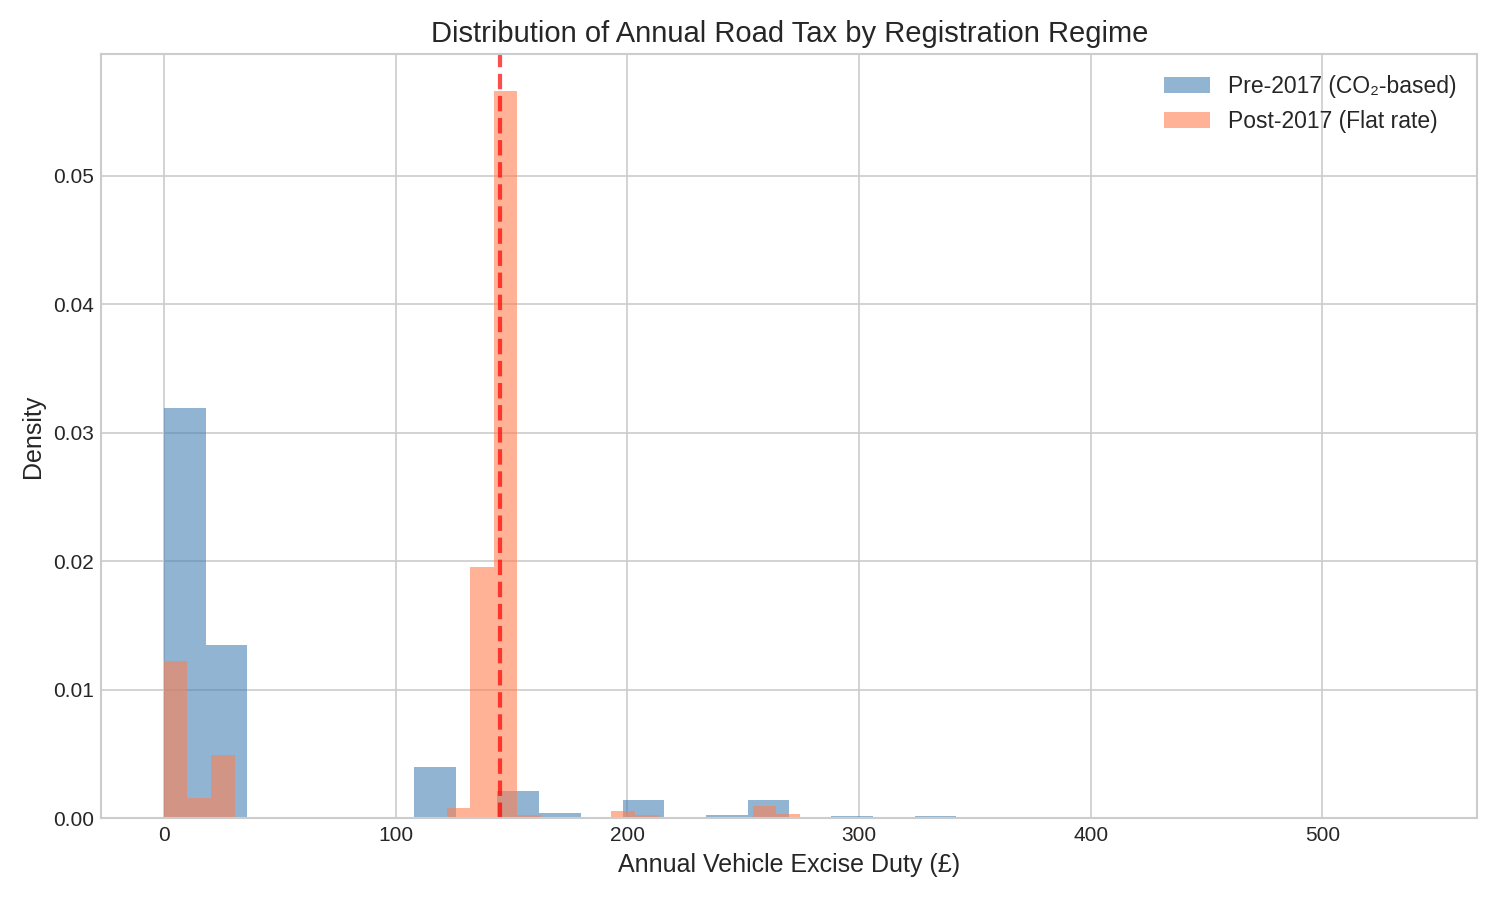
\includegraphics[width=0.75\textwidth]{tax_distribution.png}
\end{figure}
\FloatBarrier

\section{Theoretical Framework}
This section develops the economic model underlying my empirical analysis. I present a hedonic equilibrium model with explicit treatment of operating costs, then derive the structural pricing equation used for estimation.

\paragraph{Agents.}
The economy consists of a continuum of heterogeneous consumers $i \in [0,1]$ and a competitive fringe of sellers. Consumers differ in their expected holding period $T_i$, discount factor $\beta_i$, and taste parameters. Sellers offer vehicles characterised by observable attributes in a competitive secondary market.

\paragraph{Vehicle Characteristics.}
Each vehicle $j$ is characterised by a vector of attributes:
\begin{equation}
    \mathbf{x}_j = (a_j, k_j, e_j, f_j, \tau_j)
\end{equation}
where $a_j$ is vehicle age (years since first registration), $k_j$ is mileage, $e_j$ is engine size, $f_j$ is fuel type (petrol/hybrid/diesel), and $\tau_j \in \{0,1\}$ indicates the tax regime (0 = pre-April 2017, 1 = post-April 2017).

\paragraph{Utility.}
Consumer $i$'s indirect utility from purchasing vehicle $j$ at price $P_j$ is:
\begin{equation}
    U_{ij} = \underbrace{v(q_j)}_{\text{quality utility}} - \underbrace{P_j}_{\text{purchase price}} - \underbrace{C^{op}_{j}}_{\text{PV operating costs}} +   \varepsilon_{ij}
\end{equation}
where $v(q_j)$ represents utility from vehicle quality, $C^{op}_j$ is the present value of expected operating costs (including taxes), and $\varepsilon_{ij}$ captures idiosyncratic preferences.

The present value of tax costs over expected holding period $T$ with discount rate $r$ is:
\begin{equation}
    C^{tax}_{j} = \sum_{t=1}^{T} \frac{\text{VED}_j(\tau_j)}{(1+r)^t}
    = \text{VED}_j \cdot \frac{1-(1+r)^{-T}}{r},
\end{equation}
in line with asset-pricing approaches that relate automobile values to the present discounted value of operating costs \citep{kahn1986,dreyfusviscusi1995,allcottwozny2014,salleewestfan2016,grigolon2018}, where $\text{VED}_j(\tau_j)$ denotes the annual Vehicle Excise Duty, which depends on the tax regime. For pre-2017 vehicles, VED varies with CO\textsubscript{2} emissions; for post-2017 vehicles, VED is approximately constant at \pounds 145.


\paragraph{Information.}
I assume full information: all buyers observe all vehicle characteristics $\mathbf{x}_j$, the tax regime $\tau_j$, and the applicable VED schedule at the time of purchase. Sellers know the characteristics of the vehicles they offer. This assumption is reasonable given that VED rates are publicly available, vehicle specifications are listed in advertisements, and registration dates are recorded on official documents. This assumption is standard in equilibrium models of automobile demand and pricing \citep{berry1995}.

\paragraph{Enforcement.}
Property rights are fully enforced through the UK vehicle registration system administered by the DVLA. Legal ownership transfers upon sale, and VED obligations are tied to the registered keeper. There is no risk of expropriation or contract non-performance.

\paragraph{Matching.}
Buyers and sellers meet through a decentralised market (online platforms, dealerships, private sales). I assume frictionless matching, that is, any buyer can purchase any listed vehicle at the posted price. Search costs and bargaining frictions are abstracted away.

\paragraph{Market Structure.}
The used car market is assumed to be competitive with frictionless matching. Sellers are price-takers who accept the market-clearing hedonic price schedule $P(\mathbf{x})$.

\paragraph{State and Control Variables.}
From the consumer's perspective, state variables include vehicle characteristics $\mathbf{x}_j$, the tax regime $\tau_j$, and current wealth. The control variable is the discrete choice of which vehicle $j$ to purchase (or not to purchase). This is a static model of a single purchase decision; I do not model dynamic replacement or resale decisions.

\paragraph{Equilibrium.}
In a hedonic equilibrium \cite{rosen1974,bajari2005}, the price function $P^*(\mathbf{x})$ equates marginal willingness to pay with marginal cost across all characteristics. Consumers choose vehicles to maximise $U_{ij} - P(\mathbf{x}_j)$, and markets clear for each characteristic bundle. The equilibrium price reflects both the intrinsic value of vehicle attributes and the capitalised value of future operating costs.

\paragraph{Structural Pricing Equation.}
Building on the hedonic framework, I specify a structural pricing model where the equilibrium price of vehicle $j$ at vehicle age $t$ is:
\begin{equation}
    P_{jt} = \alpha_j \cdot e^{-\delta \cdot t} - \lambda \cdot \text{NPV}(Tax_j) + \varepsilon_{jt}
    \label{eq:structural}
\end{equation}
The first term, $\alpha_j \cdot e^{-\delta \cdot t}$, captures the intrinsic value of model $j$ depreciating exponentially at rate $\delta$ per year. This functional form is consistent with evidence that automobile values are well-approximated by geometric depreciation \citep{kahn1986,storchmann2004}. The second term, $\lambda \cdot \text{NPV}(Tax_j)$, represents the capitalised value of future tax liabilities, where $\lambda$ is the tax capitalisation coefficient, which is the main structural parameter of interest for this study. The error term $\varepsilon_{jt}$ captures unobserved parts for researchers due to the data limitation such as vehicle condition, local market effects, and listing-specific other factors.

The model contains two scalar parameters ($\delta$, $\lambda$) and a vector of model fixed effects ($\alpha_1, ..., \alpha_J$). The depreciation rate $\delta$ implies 10\% annual depreciation. The tax capitalisation coefficient $\lambda$ measures the extent to which consumers discount future tax liabilities into current prices. Under full rationality, $\lambda = 1$, meaning consumers value £1 of future tax liability at exactly £1 in present value terms. If $\lambda = 0$, consumers are completely myopic and ignore future taxes. Values of $\lambda > 1$ would suggest over-capitalisation, consistent with highly salient or overweighted operating-cost components discussed in the fuel-economy valuation literature \citep{allcott2014,grigolon2018,sallee2016}.
Next, the model fixed effects $\alpha_j$ capture the all time-invariant characteristics including brand positioning, reliability, fuel type, and engine specifications.

Identification of $\delta$ comes from within-model price variation across vehicle ages: older vehicles of the same model trade at lower prices, and the rate of decline identifies the depreciation parameter. Identification of $\lambda$ comes from the 2017 VED reform, which created cross-sectional variation in tax liabilities across otherwise similar vehicles. The seemingly reveral pattern, where low-emission vehicles faced tax increases while high-emission vehicles received tax cuts, is utilised for identification, as it generates variation in $\text{NPV}(Tax_j)$ that is orthogonal to unobserved quality conditional on model fixed effects.

Following the literature, I calibrate the discount rate at $r = 0.05$ (consistent with estimates of time preference and auto loan rates in car markets; \cite{dreyfusviscusi1995}) and the expected holding period at $T = 5$ years, which is broadly in line with vehicle survivability and ownership patterns documented in transportation studies \citep{lu2006}. These values imply an NPV factor of approximately 4.33, so that \pounds 100 in annual tax liability translates to \pounds 433 in present value terms.

\begin{table}[H]
\centering
\caption{Model Parameters}
\label{tab:parameters}
\begin{tabular}{cllc}
\toprule
Parameter & Description & Identification & Value \\
\midrule
$\delta$ & Annual depreciation rate & Age-price gradient & Estimated \\
$\lambda$ & Tax capitalisation coefficient & Tax-price gradient & Estimated \\
$\alpha_j$ & Model intrinsic value (FE) & Model mean prices & Estimated \\
$r$ & Discount rate & Calibrated & 0.05 \\
$T$ & Holding period (years) & Calibrated & 5 \\
\bottomrule
\end{tabular}
\end{table}

\section{Results}

This section presents the main estimation results. I first discuss the structural parameter estimates from the SMM procedure, then examine heterogeneous effects across vehicle types using machine learning methods.

Table \ref{tab:smm_results} reports the SMM estimation results. The estimated depreciation rate is $\hat{\delta} = 0.10$ with a bootstrap standard error of 0.004, implying that Toyota vehicles lose approximately 10\% of their value annually. This estimate is consistent with industry benchmarks for Toyota, which is known for strong residual values relative to other manufacturers. The depreciation parameter is estimated, and a t-statistic exceeds 20.

\begin{table}[ht]
    \centering
    \caption{Structural Estimation Results (SMM)}
    \label{tab:smm_results}
    \begin{threeparttable}
    \begin{tabular}{lcccc}
        \toprule
        Parameter & Estimate & Std. Error & t-statistic & p-value \\
        \midrule
        Depreciation rate ($\delta$) & 0.0996 & 0.0045 & 22.13 & $<$0.001 \\
        Tax capitalisation ($\lambda$) & 0.9546 & 0.5176 & 1.84 & 0.065 \\
        \midrule
        \multicolumn{5}{l}{\textit{Hypothesis Tests}} \\
        $H_0: \lambda = 0$ & \multicolumn{4}{c}{$t = 1.84$, $p = 0.065$} \\
        $H_0: \lambda = 1$ & \multicolumn{4}{c}{$t = -0.09$, $p = 0.930$} \\
        \midrule
        Model fixed effects & \multicolumn{4}{c}{15 models} \\
        Moment conditions & \multicolumn{4}{c}{74 (Model $\times$ Year)} \\
        Observations & \multicolumn{4}{c}{6,568} \\
        $R^2$ & \multicolumn{4}{c}{0.903} \\
        \bottomrule
    \end{tabular}
    \begin{tablenotes}
        \small
        \item \textit{Note:} Standard errors computed via bootstrap with 200 replications. The discount rate is calibrated at $r = 0.05$ and the holding period at $T = 5$ years.
    \end{tablenotes}
    \end{threeparttable}
\end{table}

The main parameter of interest in this study is the tax capitalisation coefficient. The point estimate is $\hat{\lambda} = 0.95$ with a standard error of $0.52$, implying that consumers capitalise approximately 95 pence of every pound of future tax liability into current vehicle prices. I test two null hypotheses of economic interest. First, I test the null of no capitalisation ($\lambda = 0$) and obtain $t = 1.84$ and $p = 0.065$. Thus, I reject $\lambda = 0$ at the 10\% significance level, providing suggestive evidence against complete consumer myopia. However, this result is not statistically significant at the conventional 5\% level, and, given that the analysis is based on a single brand with relatively imprecise estimates, it should be interpreted with caution. Second, I cannot reject the null of full capitalisation ($\lambda = 1$), so the data are consistent with consumers approximately fully capitalising future tax liabilities into current prices. The 95\% confidence interval of $[-0.06, 1.97]$ includes unity. These results suggest that UK used car buyers behave approximately as rational agents who fully incorporate future tax obligations into their purchase decisions.

To illustrate the economic magnitude, I consider the tax differential for a Toyota Prius. A pre-2017 Prius qualifies for \pounds 0 annual tax, while a post-2017 model faces \pounds 135 per year, implying a present value difference of approximately \pounds 585 over a five-year holding period. With $\hat{\lambda} = 0.95$, this translates to a price premium of roughly \pounds 556 for pre-2017 Prius models relative to otherwise identical post-2017 counterparts. Conversely, high-emission vehicles like the GT86 experienced tax reductions under the new regime, and should therefore command higher prices in post-2017 vintages.

\begin{figure}
    \centering
    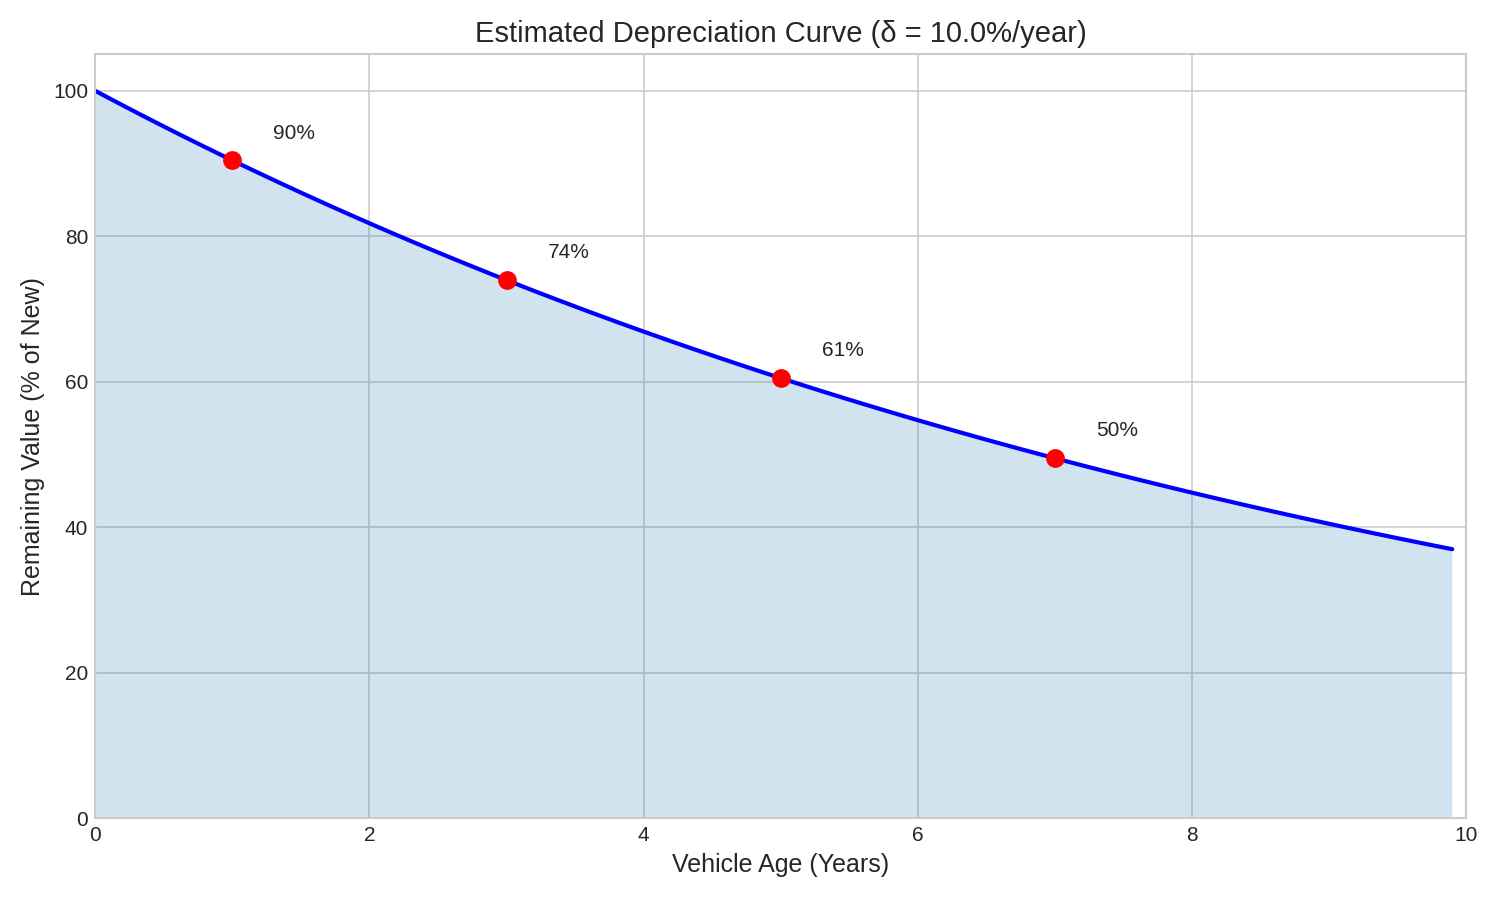
\includegraphics[width=0.75\linewidth]{depreciation_curve.png}
\end{figure}

\FloatBarrier


\paragraph{Heterogeneity Analysis.}
While the SMM estimation provides an average capitalisation rate, it assumes a constant $\lambda$ across all vehicles. However, the 2017 reform was structurally asymmetric: it penalised low-emission vehicles (which lost their tax exemption) while effectively subsidising high-emission vehicles (whose tax liabilities were capped). To examine whether price responses varied systematically across vehicle types, I employ a machine learning approach to estimate heterogeneous treatment effects.

Specifically, I implement a Random Forests (RF), following the causal forest literature \citep{athey2016, wager2018}
. The approach proceeds in two steps. First, I train a RF on pre-2017 vehicles to learn the relationship between vehicle characteristics and prices under the old tax regime. The feature set includes age, mileage, engine size, and transmission type. Second, I use this model to predict counterfactual prices for post-2017 vehicles (what their prices would have been under the pre-2017 tax structure). The estimated price shock for each vehicle is:
\begin{equation}
    \hat{\tau}_i = P_i^{obs} - \hat{E}[P_i | X_i, \text{Regime} = \text{Pre-2017}]
\end{equation}
A positive $\hat{\tau}_i$ indicates that the vehicle trades at a premium relative to one of pre-2017 pricing structure would predict. A negative value indicates a discount.

\begin{table}[ht]
    \centering
    \caption{Estimated Price Impact by Model}
    \label{tab:hetero_impact}
    \begin{threeparttable}
    \begin{tabular}{llccc}
        \toprule
        Model & Type & Avg. MPG & N & Price Impact ($\hat{\tau}$) \\
        \midrule
        Land Cruiser & SUV & 32.2 & 31 & +\pounds 12,450 \\
        GT86 & Sports & 34.6 & 53 & +\pounds 7,232 \\
        Corolla & Family & 64.5 & 257 & +\pounds 6,214 \\
        C-HR & Crossover & 66.1 & 471 & +\pounds 5,778 \\
        Prius & Hybrid & 80.8 & 101 & +\pounds 4,868 \\
        Auris & Hatchback & 68.9 & 278 & +\pounds 155 \\
        Yaris & City & 59.1 & 1,383 & +\pounds 53 \\
        Avensis & Saloon & 56.6 & 45 & +\pounds 26 \\
        \bottomrule
    \end{tabular}
    \begin{tablenotes}
        \small
        \item \textit{Note:} Price impact represents the average difference between observed prices and counterfactual prices predicted by a Random Forest model trained on pre-2017 data. Positive values indicate the vehicle trades at a premium relative to the pre-2017 pricing structure.
    \end{tablenotes}
    \end{threeparttable}
\end{table}

Table \ref{tab:hetero_impact} reports the estimated price impacts by model, sorted by magnitude. The results reveal substantial heterogeneity consistent with the reversal pattern implied by the reform. High-emission vehicles that previously faced punitive tax rates experienced the largest positive valuation shocks. The Land Cruiser, a large SUV with average fuel economy of just 32 MPG, shows a price premium of over \pounds 12,000 relative to counterfactual. The GT86 sports car, with similarly poor fuel efficiency, gained approximately \pounds 7,200. These vehicles benefited most from the flat-rate cap, which reduced their lifetime tax burden in large amount.

These findings have important policy implications. While the 2017 reform successfully addressed the fiscal problem, it simultaneously created perverse incentives in the used car market. By capping the tax liability of high-emission vehicles, the reform effectively subsidised continued ownership of the most polluting vehicles, undermining the environmental objectives that motivated the original CO\textsubscript{2}-based system.

\begin{figure}
    \centering
    
\includegraphics[width=0.75\linewidth]{tax_by_fueltype.png}
\end{figure}

\begin{figure}
    \centering
    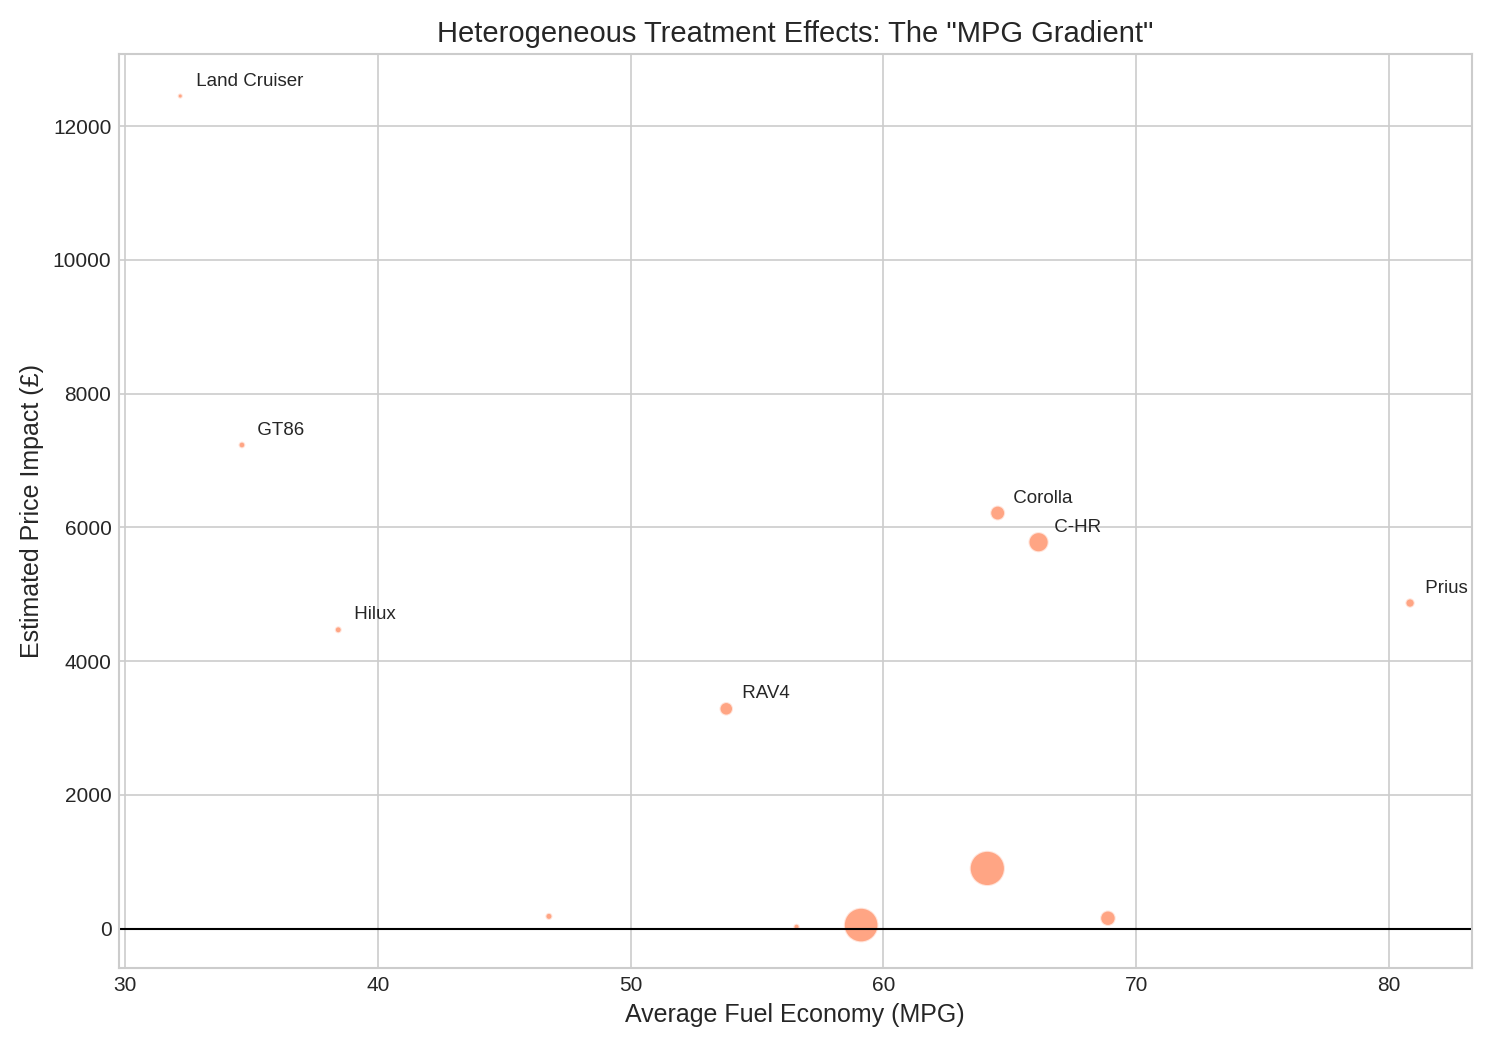
\includegraphics[width=0.75\linewidth]{heterogeneity_mpg.png}
\end{figure}

\FloatBarrier

\section{Conclusion and Discussion}
This paper examines the extent to which UK consumers capitalise vehicle taxes into used car prices, leveraging the April 2017 Vehicle Excise Duty reform as a natural experiment. Using Simulated Method of Moments (SMM) estimation with a structural pricing model, I find a tax capitalisation coefficient of approximately 0.95, which is statistically indistinguishable from unity. This result implies that consumers behave as approximately rational agents who fully incorporate future tax obligations into their vehicle purchase decisions. The finding contributes to the tax salience literature by demonstrating that even recurring annual taxes are efficiently priced into durable goods markets.

The 2017 reform was primarily motivated by fiscal concerns. Under the pre-2017 CO\textsubscript{2}-based system, improvements in vehicle technology had progressively eroded the tax base as an increasing share of vehicles qualified for low or zero tax rates. Government projections indicated that over three-quarters of new vehicles would pay no first-year tax by 2017, threatening significant revenue losses. The shift to a flat-rate standard charge successfully addressed this problem by broadening the tax base. My empirical results confirm that post-2017 versions of previously tax-exempt vehicles, such as the Toyota Yaris and Prius, now trade at lower prices relative to their pre-2017 counterparts, reflecting the increased cost of ownership under the new regime.

However, the heterogeneity analysis reveals an unintended consequence of the reform. While low-emission vehicles lost their tax advantage, high-emission vehicles received effective tax relief. Under the pre-2017 system, vehicles with emissions above 200 g/km faced annual taxes exceeding £300, and in some cases over £500. The flat-rate system caps these liabilities at approximately £145 per year, substantially reducing the lifetime tax burden for the most polluting vehicles. The T-Learner results show that high-emission models such as the Land Cruiser and GT86 experienced positive valuation shocks of several thousand pounds, as the market priced in their reduced future tax obligations. In contrast, fuel-efficient vehicles gained little or saw their relative values decline.

This asymmetric price response has implications for environmental policy. The original CO\textsubscript{2}-based system was designed to discourage ownership of high-emission vehicles by imposing higher operating costs. By removing this differentiation, the 2017 reform inadvertently subsidised the continued ownership of polluting vehicles in the secondary market. The positive price premium for high-emission vehicles may encourage consumers to retain or purchase these models rather than switching to more efficient alternatives. This outcome contradicts the environmental objectives that motivated the introduction of emissions-based taxation in 2001.

Several limitations of this study need to be addressed. First, the dataset contains asking prices rather than final transaction prices, which may introduce measurement error if negotiation patterns differ systematically across vehicle types. Second, the year variable represents model year rather than registration date, and since the VED regime is determined by registration date, this creates attenuation bias that may cause the capitalisation coefficient to be underestimated. Third, the analysis is limited to Toyota vehicles, and results may not generalize to other manufacturers with different brand positioning or customer demographics. Fourth, it is more static analysis and does not show the dynamic responses to the reform over time.

Future research could address these limitations by obtaining transaction-level data with precise registration dates, extending the analysis to multiple manufacturers, and examining how capitalisation rates evolve as consumers learn about the new tax structure. Additionally, incorporating data on fuel prices would allow separate identification of fuel cost and tax cost capitalisation, providing a more complete picture of how consumers value vehicle operating costs.

\begin{thebibliography}{9}

\bibitem{allcott2014}
Allcott, H., and Wozny, N. (2014).
``Gasoline Prices, Fuel Economy, and the Energy Paradox.''
\textit{Review of Economics and Statistics}, 96(5): 779--795.

\bibitem{athey2016}
Athey, S., and Imbens, G. (2016).
``Recursive Partitioning for Heterogeneous Causal Effects.''
\textit{Proceedings of the National Academy of Sciences}, 113(27): 7353--7360.

\bibitem{bajari2005}
Bajari, P., and Benkard, C. L. (2005).
``Demand Estimation with Heterogeneous Consumers and Unobserved Product Characteristics: A Hedonic Approach.''
\textit{Journal of Political Economy}, 113(6): 1239--1276.

\bibitem{berry1995}
Berry, S., Levinsohn, J., and Pakes, A. (1995).
``Automobile Prices in Market Equilibrium.''
\textit{Econometrica}, 63(4): 841--890.

\bibitem{busse2006}
Busse, M., Silva-Risso, J., and Zettelmeyer, F. (2006).
``$1{,}000$ Cash Back: The Pass-Through of Auto Manufacturer Promotions.''
\textit{American Economic Review}, 96(4): 1253--1270.

\bibitem{CerrutiAlberiniLinn2017}
Cerruti, D., Alberini, A., and Linn, J. (2017).
``Charging Drivers by the Pound: The Effects of the UK Vehicle Tax System.''
\textit{CER-ETH Economics Working Paper} No.~17/271, ETH Zurich.

\bibitem{chetty2009}
Chetty, R., Looney, A., and Kroft, K. (2009).
``Salience and Taxation: Theory and Evidence.''
\textit{American Economic Review}, 99(4): 1145--1177.

\bibitem{dvla2001}
Driver and Vehicle Licensing Agency (DVLA). (2001).
\textit{Vehicle Excise Duty Rates Based on CO\textsubscript{2} Emissions}.
UK Department for Transport.

\bibitem{dvla2015}
Driver and Vehicle Licensing Agency (DVLA). (2015).
\textit{Vehicle Excise Duty Statistics}.
UK Department for Transport.

\bibitem{dvla2017}
Driver and Vehicle Licensing Agency (DVLA). (2017).
\textit{Vehicle Excise Duty: 2017 Reform Overview and Rate Tables}.
UK Department for Transport.

\bibitem{dreyfusviscusi1995}
Dreyfus, M. K., and Viscusi, W. K. (1995).
``Rates of Time Preference and Consumer Valuations of Automobile Safety and Fuel Efficiency.''
\textit{Journal of Law and Economics}, 38(1): 79--105.

\bibitem{finkelstein2009}
Finkelstein, A. (2009).
``E-ZTAX: Tax Salience and Tax Rates.''
\textit{Quarterly Journal of Economics}, 124(3): 969--1010.

\bibitem{grigolon2018}
Grigolon, L., Reynaert, M., and Verboven, F. (2018).
``Consumer Valuation of Fuel Costs and Tax Policy: Evidence from the European Car Market.''
\textit{American Economic Journal: Economic Policy}, 10(3): 193--225.

\bibitem{hmt2015}
HM Treasury. (2015).
\textit{Summer Budget 2015}.
London: Her Majesty's Treasury.

\bibitem{ifs2019}
Adam, S., and Stroud, R. (2019).
``A Road Map for Motoring Taxation.''
\textit{Institute for Fiscal Studies}.

\bibitem{kahn1986}
Kahn, J. A. (1986).
``Gasoline Prices and the Used Automobile Market: A Rational Expectations Asset Price Approach.''
\textit{Quarterly Journal of Economics}, 101(2): 323--339.

\bibitem{lu2006}
Lu, S. (2006).
\textit{Vehicle Survivability and Travel Mileage Schedules.}
National Highway Traffic Safety Administration, National Center for Statistics and Analysis.

\bibitem{oates1969}
Oates, W. E. (1969).
``The Effects of Property Taxes and Local Public Spending on Property Values: An Empirical Study of Tax Capitalization and the Tiebout Hypothesis.''
\textit{Journal of Political Economy}, 77(6): 957--971.

\bibitem{rac2017}
RAC Foundation. (2017).
\textit{Fuel for Thought: The What, Why and How of Motoring Taxation}.

\bibitem{rosen1974}
Rosen, S. (1974).
``Hedonic Prices and Implicit Markets: Product Differentiation in Pure Competition.''
\textit{Journal of Political Economy}, 82(1): 34--55.

\bibitem{sallee2016}
Sallee, J. M., West, S. E., and Fan, W. (2016).
``Do Consumers Recognize the Value of Fuel Economy? Evidence from Used Car Prices and Gasoline Price Fluctuations.''
\textit{Journal of Public Economics}, 135: 61--73.

\bibitem{storchmann2004}
Storchmann, K. (2004).
``On the Depreciation of Automobiles: An International Comparison.''
\textit{Transportation}, 31(4): 371--408.

\bibitem{ukbudget1999}
HM Treasury. (1999).
\textit{Budget 1999: Stability and Steady Growth for Britain}.
London: Her Majesty’s Treasury.

\bibitem{wager2018}
Wager, S., and Athey, S. (2018).
``Estimation and Inference of Heterogeneous Treatment Effects Using Random Forests.''
\textit{Journal of the American Statistical Association}, 113(523): 1228--1242.



\end{thebibliography}
\end{document}